


\newcommand{\gwb}{g_\text{1}}
\newcommand{\gva}{g_\text{2a}}
\newcommand{\gvb}{g_\text{2b}}
\newcommand{\ghf}{g_\text{3}}
\newcommand{\gd}{g_\text{4}}
\newcommand{\gta}{g_\text{5a}}
\newcommand{\gtb}{g_\text{5b}}
\newcommand{\gca}{g_\text{6}}
\newcommand{\gzb}{g_\text{7}}


\begin{figure}[H]
	\centering
	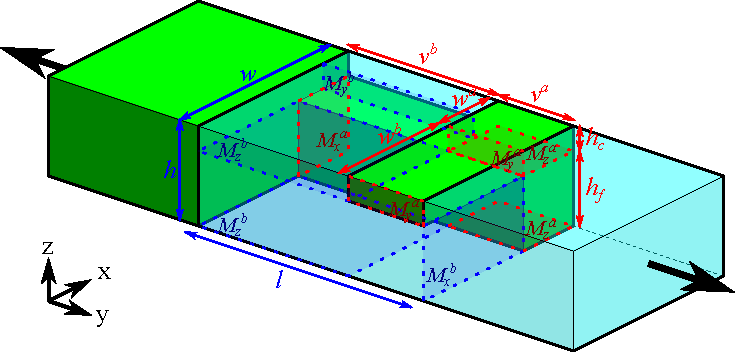
\includegraphics[width=\columnwidth]{sources/method/straight_model_v3.pdf}
	\caption{
		One straight unit cell connecting material $a$ (left) to material $b$ (right).
		Failure can happen along the fingers ($M_x$), along the cross beams ($M_y$) or at the interface between the two ($M_z$) for either material.}
	\label{fig:failure_modes}
\end{figure}


\section{Straight design}



\Cref{fig:failure_modes} shows one cell of the straight design, along with the design variables and the failure modes.
The aim is to optimize the effective ultimate tensile strength while keeping the perpendicular area of the structure minimal.
Variables $\wb$, $\va$, $\vb$, $\hf$ and $F$ will be optimized.


\subsection{Problem Formulation}
This section shows the derivation of the optimization problem. 

\subsubsection{Tension Failure M\textsubscript{x}}
The tensile stresses in the fingers of either material $m$ are computed with $\frac{F}{A}$ as shown in \cref{eq:tens}.
\begin{align}\label{eq:tens}
	\sigma_{11}^m &= \frac{ F }{ w^m \hf }
\end{align}

\subsubsection{Shear Failure M\textsubscript{y}}
The shear stresses $\frac{F}{A}$ acting on $M_y^m$ for either material $m$ are determined by modeling the the cross beam as a cantilever beam fixed at both ends.
The load is modeled as a uniformly distributed load over the whole beam.
Because the beam is fixed on both sides, the shear force equals half the total force acting on the beam as shown in \cref{eq:sh}.

The parameter $d_y^m$ indicates the portion of the total force $F$ which acts upon the unsupported part of material $a$ and is proportional to $\wb / w$, where $w = \wa+\wb$ as given in \cref{eq:dy}.
However, in some cases the full force acts on the beam which will be discussed later.  
To select between these case, the parameter $u_y^m$ can be varied between 0 and 1.

\begin{align}\label{eq:sh}
	\sigma_{13}^m &= \frac{d_y^m F}{2 v^m \hc} 
\end{align}
\begin{align}\label{eq:dy}
	d_y^m &= \frac{w^{\neg m} + u_y^m w^m}{w}
\end{align}

\subsubsection{Bending Failure M\textsubscript{y}}

The highest bending stress for a doubly supported beam occurs in the middle and is given in \cref{eq:bs}.
\begin{align}\label{eq:bs}
	\sigma_{22}^m &= \frac{M}{I}c = \frac{d_y^m F w^{\neg m} / 12}{\hc (v^m)^3 / 12} \nicefrac12 v^m 
	=  \frac{ d_y^m F w^{\neg m} }{ 2 \left( v^m \right)^2 \hc }
	= \sigma_{13}^m \frac{w^{\neg m}}{v^m}
\end{align}

\subsubsection{Shear Failure M\textsubscript{z}}
There is also a shear stress acting on the surface $M_z^m$.
On the one hand one might think that only a portion $d_z^m$ of the total force $F$ is acting on the supported portion of the cross beam.
On the other hand the total force must be enacted through this plane, because it is the only connection between the finger and the cross beam.
The term $u_z^m$ switches between a fraction of and the full force by varying it in between 0 or 1 respectively.
In order to compare the stresses along the Z direction and stresses along the XY direction against the same ultimate stress value $\sigmafail$, the Z shear stress was multiplied with the ratio $\nicefrac{\sigmafail}{\sigmafailz}$.
The shear stress along Z is therefore given in \cref{eq:mz}
\begin{align}\label{eq:mz}
	\sigma_{12}^m &= \frac{\sigmafail}{\sigmafailz} \frac{ d_z^m F }{ 2 v^m w^m} \\ 
	d_z^m &= \frac{w^m + u_z^m w^{\neg m}}{w}
\end{align}

\subsubsection{Optimization Problem}
Based on the stresses derived above, the following optimization problem was obtained.
% The naive model will be fine-tuned and several variants will be considered.
% Finally we compare the variants against experimental FEM simulation results in order to get to the final formulation of the optimization problem.
% \footnote{Even though finding the correct model is not the focus of this course, it is relevant to my PhD research and we cover several interesting ideas pertaining to engineering optimization.}

\begin{align}
	f:& \omit\rlap{$\displaystyle \max{ \frac{F}{\left( \wa + \wb \right) \left( \hf + \hc \right) }}$} \label{eq:obj} \\
	\omit\rlap{subject to} \nonumber \\
	\gwb: & w^m \ge 2 \wmin^m		&&	\text{ Nozzle size} \label{eq:c1} \\
	g_2: & v^m \ge \wmin^m			&&	\text{ Nozzle size}  \label{eq:c2} \\
	g_{3f}: &\hf \ge \hmin	&&	\text{Layer thickness}  \label{eq:c3} \\
	g_{3c}: & \hc \ge \hmin	&&	\text{Layer thickness}  \label{eq:c4} \\
	\gd: & \va + \vb \le \Lmax      &&   \text{ Design constraint}   \label{eq:c_total_length} \\
	g_5: & \sigma_{11}^m = \frac{ F }{ w^m \hf } \le \sigmafail^m				&&	\text{ Tension failure } M_x^m  \label{eq:c_tensile} \\
	g_{6,S}: & \sigma_{13}^m = \frac{ F w^{\neg m} }{ 2 v^m \hc w } \le \taufail^m			&&		\text{ Shear failure } M_y^m  \label{eq:c_shear} \\
	g_{6,B}: & \sigma_{22}^m = \frac{ F \left(w^{\neg m}\right)^2 }{ 2 \left( v^m \right)^2 \hc w } \le \sigmafail^a             &&    \text{ Bending failure } M_y^m  \label{eq:c_bending} \\
	\gzb: &\sigma_{12}^m = \frac{ F }{ 2 v^m w^m} \le \tauz^m						&&	\text{ Shear failure } M_z^m  \label{eq:c_shear_z} \\
	& \omit\rlap{for both materials $m \in \{a, b\}$ where $\neg a = b$ and $\neg b = a$}\nonumber
\end{align}


While the $v^m$ variables do not appear in the objective function, they are included in the constraints are therefore also subject to the optimization. 
These are bounded by the active constraints.

The constraint values depend on the printer and the materials.
Different nozzles and layer thickness settings require other limits on the design.
Due to the manufacturing constraints, the layer thickness shall be smaller than half the smallest nozzle diameter:
$\hmin < \nicefrac{1}{2} \wmin^m$.

Material properties of 3D printed materials have $\tauz^m < \taufail^m$, since the shear strength parallel to the layers is lower due to the layer bonding.


\subsubsection{Vom Mises Yield Criterion}
From the von Mises yield criterion it is known that $\taufail^m = \sigmafail^m / \sqrt{3} $.
If $\nicefrac{\wb}{\va} > \nicefrac{ \sigmafail^a }{ \taufail^a } = \sqrt{3}$, then 
$
\frac{ d_y^m F \wb }{ 2 \left( \va \right)^2 \hc \sigmafail^a}
> \frac{ d_y^m F }{ 2 \va \hc \taufail^a} 
$. 
This means that the shear failure constraints \cref{eq:c_shear} for material $a$ are dominated by the bending failure constraint \cref{eq:c_bending}.
Otherwise the latter is dominated by the former.
The same holds conversely with the materials $a$ and $b$ swapped.
Therefore, constraints \cref{eq:c_shear,eq:c_bending} can be combined.

\begin{align}\label{eq:shear_bend_combined}
	%\frac{ d_y^m F }{ 2 v^m \hc} &\le \taufail^m \\
	%\frac{ d_y^m F }{ 2 v^m \hc} &\le \nicefrac1{\sqrt{3}} \sigmafail^m \\
	%\frac{ d_y^m F }{ 2 \cdot \sqrt{3} v^m \hc} &\le \sigmafail^m \\
	%???\frac{ d_y^m F \wb }{ 2 \left( \va \right)^2 \hc } &\le \sigmafail^a \\
	%\\
	\frac{ d_y^m F }{ 2 \va \hc }  \max{\left( \sqrt{3}, \frac{\wb}{ \va} \right)} &\le \sigmafail^a  \nonumber \\
	\frac{ d_y^m F }{ 2 \vb \hc }  \max{\left( \sqrt{3}, \frac{\wa}{ \vb} \right)} &\le \sigmafail^b  
\end{align}

The same result was obtained when using the Von Mises yield criterion directly with the shear stress $\sigma_{13}$ and the bending stress $\sigma_{22}$ \cref{eq:shear_bend_von_mises}.
% The shear and bending both act on the and thereby lower the force at which failure happens.

\begin{align*}
	\left(\sigma_{11} - \sigma_{22}\right)^2  +  \left(\sigma_{22} - \sigma_{33}\right)^2  +  \left(\sigma_{33} - \sigma_{11}\right)^2  \\
	+   6\left(\sigma_{23}^2 + \sigma_{13}^2 + \sigma_{12}^2\right) &< 2 \sigmafail^2 \\
\end{align*}


\begin{align}\label{eq:shear_bend_von_mises}
	% \sqrt{ \left(  \frac{ d_y^m F \wb }{ 2 \left( \va \right)^2 \hc }  \right)^2   +   3 \left(  \frac{ d_y^m F }{ 2 \va \hc}  \right)^2 } &< \sigmafail^a \\
	% \sqrt{ \left(  \frac{ d_y^m F }{ 2 \va \hc} \frac{\wb}{\va}  \right)^2   +   3 \left(  \frac{ d_y^m F }{ 2 \va \hc}  \right)^2 } &< \sigmafail^a \\
	% \sqrt{ \left(  \frac{ d_y^m F }{ 2 \va \hc}\right)^2  \left( \frac{\wb}{\va}  \right)^2   +   3 \left(  \frac{ d_y^m F }{ 2 \va \hc}  \right)^2 } &< \sigmafail^a \\
	% \sqrt{ \left(  \frac{ d_y^m F }{ 2 \va \hc}\right)^2  \left( \left( \frac{\wb}{\va}  \right)^2   +   3  \right) } &< \sigmafail^a \\
	\sigma_{13,22}^a = \frac{ d_y^m F }{ 2 \va \hc} \sqrt{   \left( \frac{\wb}{\va}  \right)^2 + 3 } &< \sigmafail^a \nonumber \\
	\sigma_{13,22}^b = \frac{ d_y^m F }{ 2 \vb \hc} \sqrt{   \left( \frac{\wa}{\vb}  \right)^2 + 3 } &< \sigmafail^b 
\end{align}

This von Mises yield criterion \cref{eq:shear_bend_von_mises} is equivalent to the application of the P-norm smooth approximation of the maximum function as used in the combined constraint \cref{eq:shear_bend_combined}, for $P=2$.

Where $\nicefrac{\wb}{\va} \to 0$ and $\nicefrac{\wb}{\va} \to \infty$ the failure is dominated by shear and bending respectively. 
This shows that in the limits the von Mises yield criterion and the combined criterion coincide.


Similarly the tensile failure $M_x$ and shear failure $M_z$ can be combined with the von Mises criterion into $\sigma_{11,12}$.
And also for Z shear failure $M_z$ and cross beam failure $M_y$, including bending: $\sigma_{12,13,22}$; or without: $\sigma_{12,13}$.
One might even consider a combined von Mises constraint for all stresses together: $\sigma_{11,12,13,22}$.

\subsubsection{Constraint validity}
A careful analysis of the geometry will show that if shearing failure mode $M_x^a$ has occurred, 
there is still interlocking between the two materials. 
If for example a part of the cross beams of $b$ has sheared off, still a column of material $a$ remains, which is surrounded by material $b$.
Once one of those failure modes has occurred, still any other failure mode has to occur for the interlock to fail, except $M_x^b$.
Therefore a constraint was added to the shearing failure modes that both those failure modes shall occur together.
The constraint is violated only when both occur, so it is satisfied when either failure mode is prevented.
The logical disjunction can be rewritten into a minimum when both constraints are transformed into negative null form:
\begin{align*}
	% \min \left(  \frac{ d_y^m F }{ 2 \va \hc \sigmafail^a} \sqrt{   \left( \frac{\wb}{\va}  \right)^2 + 3 }  ,  \frac{ F }{ 2 \vb \hc \sigmafail^b} \sqrt{   \left( \frac{\wa}{\vb}  \right)^2 + 3 }  \right) - 1 &< 0 \\
	% \frac{ d_y^m F }{ 2 \hc}  \min \left(  \frac{ 1 }{ \va \sigmafail^a} \sqrt{   \left( \frac{\wb}{\va}  \right)^2 + 3 }  ,  \frac{ 1 }{ \vb \sigmafail^b} \sqrt{   \left( \frac{\wa}{\vb}  \right)^2 + 3 }  \right) - 1 &< 0 \\
	\frac{ d_y^m F }{ 2 \hc}  \min \left(  \frac{ \sqrt{   \left( \frac{\wb}{\va}  \right)^2 + 3 } }{ \va \sigmafail^a}   ,  \frac{  \sqrt{   \left( \frac{\wa}{\vb}  \right)^2 + 3 } }{ \vb \sigmafail^b}  \right) - 1 &< 0 \\
	% \frac{ d_y^m F }{ 2 \hc}  \min \left(  \frac{ \sqrt{   \left(\wb\right)^2 + 3 \left(\va\right)^2 } }{ \left(\va\right)^2 \sigmafail^a}   ,  \frac{  \sqrt{   \left(\wa\right)^2 + 3 \left(\vb\right)^2 } }{ \left(\vb\right)^2 \sigmafail^b}  \right) - 1 &< 0 \\
\end{align*}

Depending on the optimization algorithm used, the min operator might need to be replaced by smooth versions.
The choice between P-norm, Kreisselmeier-Steinhauser function or any of the other alternatives might be decided by properties of their derivatives.
The height of the $P$ value will determine the approximation error.
The approximation error of the max function means that the approximated constraint is more strict than the underlying sub-constraints, 
while the smooth approximation of the min function is more lenient.
This means that using a smooth approximation of this constraint could result in infeasible designs according to the analytical constraint.

Because the elongation at failure for PP is much higher than for TPLA, it is expected that in case both cross-beams break, PLA will break before PP.
Therefore, the situation can be considered where the cross beam shear constraint of material $a$ is violated and the structure will be optimized while adhering to the cross beam shear constraint of material $b$.
See \cref{fig:straight_model_broken}.
In this situation the cross beam shear and bending constraints for material $a$ do not hold.
Note that after the failure mode occured, the total force cannot be uniformly distributed over the whole length $w$, and therefore:
$
u_y^a = \text{N/A};
u_y^b = 1 ;
u_z^a = 1 ;
u_z^b = 1
$.

\begin{figure}[H]
	\centering
	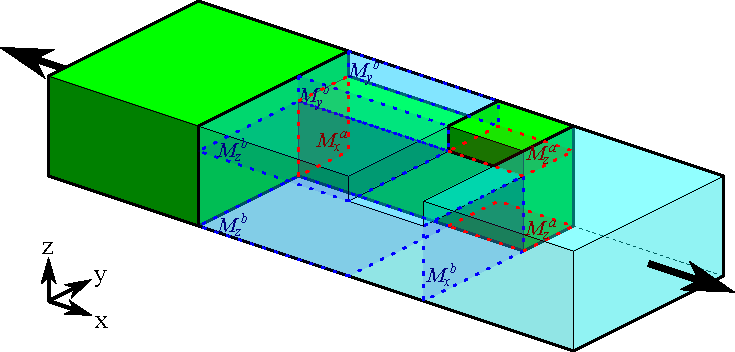
\includegraphics[width=\columnwidth]{sources/method/straight_model_v3_broken.pdf}
	\caption{The straight design if a part of the cross beam has sheared off at $M_y^a$.}
	\label{fig:straight_model_broken}
\end{figure}

All constraints containing the term $d_y^m$ can be combined into a single constraint with the following scheme:
\begin{align*}
	\begin{array}{l}
		h_1(\mathbf{x}) < 0 \\
		\vdots \\
		h_N(\mathbf{x}) < 0 \\
	\end{array}
	\to
	\max \left(h_1(\mathbf{x}), \dots, h_N(\mathbf{x}) \right) < 0
\end{align*}
By using a smooth version of the $\max$ function like described above can overcome undifferentiability issues.
However, combining all constraints into a single constraint reduces the understanding and analysis possibilities of a particular point in the design space. 


\subsubsection{Model Validation}
When subjecting the microstructure to a load the distribution of stress is difficult to predict because of the interplay between several failure modes.
The current model makes assumptions on the homogeneity of the stress distribution throughout the beams.
Several modeling choices that were deferred have been mentioned: the values for $u^m_y$, $u^m_z$, the exclusion of the bending constraints and using the combined von Mises criterions.
In order to evaluate which analytical model is the most representative, the results of an extensive grid search were compared to FEM simulations.
\footnote{The FEM simulations were not performed by either of the two students that contributed to this report. 
	Therefore the implementation details of the FEM simulation are left out.}

The grid search was performed along three dimensions: $\wb$, $\va$ and $\hf$, within the ranges $(0.6,3.0)$, $(0.1\Lmax, 0.9\Lmax)$ and $(1.8, 3.6)$ respectively.
Because the design constraint is active, and also the minimum feature size is active, $\wa$, $\vb$ and $\hc$ can be derived.
The output of each simulation is a force $F$ which can be used to compute the ultimate tensile strength $f$ of a given design.

Similarly the problem was converted such that for each design in the 3D space, the force is computed according to each mechanical constraint.
For example, the minimum force according to the tensile constraint for $a$ would be $F = \sigmafail^a \wa \hf$.
Because the structure fails as soon as the first mechanical constraint is violated, the minimum force for all constraints is recorded and used to compute the predicted ultimate strength.
Also for the comparison, $\sigmafailz^m$ was set equal to $\sigmafail^m$ because the FEM simulations cannot anisotropic material behaviour when there is a difference in strength along the Z direction caused by the layerwise buildup of FDM 3D printing.

\begin{table}[h]
	\centering
	\caption{Accuracy of the analytical model w.r.t. FEM results.}
	\label{tab:prediction_ratios}
	\begin{tabular}{llll|ll}
		$u^m_z$ & $\sigma_{22}$ & $\sigma_{11,12}$ & $\sigma_{12,13}$ & $\nicefrac{F}{\hat{F}}$ & std dev \\
		\hline
		\checkmark & - & - & - & 104.2\% & 19.8\% \\
		\checkmark & - & - & \checkmark & 101.7\% & 18.9\% \\
		\checkmark & - &\checkmark&\checkmark & 94.7\% & 19.3\% \\
		\checkmark & - &\checkmark& - & 97.0\% & 20.5\% \\
		\checkmark &\checkmark& - & - & 85.3\% & 31.0\% \\
		- & - & - &\checkmark& 107.6\% & 16.2\% \\
		- & - & - & - & 107.8\% & 16.2\% \\
	\end{tabular}
\end{table}

Each point in the FEM data set was compared to the analytical model,
and the average prediction ratio $\nicefrac{F}{\hat{F}}$ between the simulated $\hat{F}$ and the analytically predicted $F$ was calculated, along with the standard deviation as shown in \cref{tab:prediction_ratios}.
From these results it can be observed that including the bending stress $\sigma_{22}$ does not improve the accuracy of the analytical model.
Also the $\sigma_{11,12}$ von Mises criterion which combines tensile and Z shear lowers the accuracy.
Using the $\sigma_{12,13}$ von Mises criterion to combine the stresses in the cross beam with the Z shear stress does improve the model.

The question whether the full force should be used to compute the Z shear stress $u^m_z$ is more difficult to answer;
while the prediction ratio gets closer to \SI{100}{\percent}, the standard deviation increases.
It makes sense that the analytical model overestimates the ultimate strength since homogenous stress distributions are assumed.
Omitting $u^m_z$ may cause an increase in the prediction ratio, but the overall shape is closer to the FEM predictions as indicated by the lower standard deviation.
Because the actual ultimate strength is less of a concern compared to obtaining the optimal design, it was chosen to only use the partial force when computing the Z shear stress.

The comparison on the final model is shown in \cref{fig:ana_vs_FEM}.
The correct value for $\sigmafailz^m$ was set and the analytical model was evaluated on a more dense grid.
See \cref{fig:ana_minF}.
One important observation is that four constraint surfaces can be distinguished which culminate in the same optimum, while there are only three free design variables.
The four surfaces meet in a three-dimensional space, however this is not a coincidence but is presumably inherent to the particular problem at hand.

When evaluating the converted analytical model it was verified that all domain constraints are met. 
In this way, it was confirmed that the value for $\wa$ and $\hc$ can be assumed as in \cref{sec:domain_assumptions}.
Since none of the other design variables are below their lower bound, it could be concluded that these two variables had to be at their lower bound rather than any of the others.


\begin{figure}[h]
	\centering
	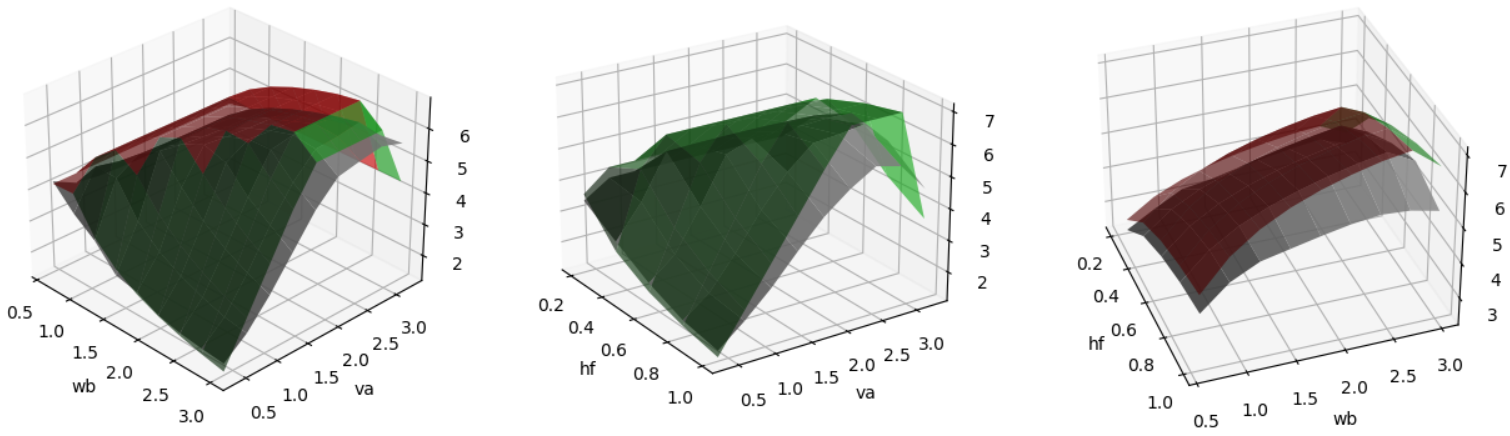
\includegraphics[width=\columnwidth]{sources/method/ana_vs_FEM.png}
	\caption{Ultimate tensile strength, colored according to failure mode and FEM simulation results in gray.
		These are three 2D slices through the 3D space spanned by $\wb$, $\va$ and $\hf$, sliced at the maximum ultimate strength value.
	}
	\label{fig:ana_vs_FEM}
\end{figure}



\begin{figure}[h]
	\centering
	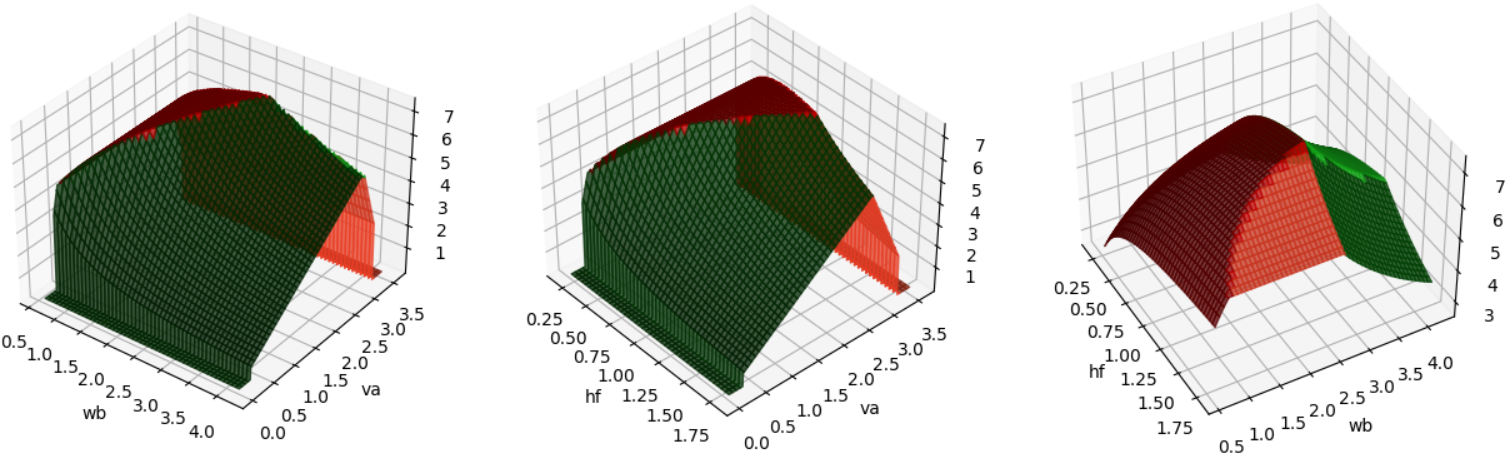
\includegraphics[width=\columnwidth]{sources/method/ana_minF.png}
	\caption{Ultimate tensile strength, colored according to failure mode according to the validated model.
		These are three 2D slices through the 3D space spanned by $\wb$, $\va$ and $\hf$, sliced at the maximum ultimate strength value.
	}
	\label{fig:ana_minF}
\end{figure}


%\todo{TODO: rescale objective function so that they are approximately in the range 0-1.}

%\todo{TODO: should we invert the mechanical constraints, so that the F is below the division line?}


\subsubsection{Problem Reformulation}
Based on the findings as mentioned above, the design problem was reformulated to the negative null form.
The shear constraints were combined into one.
The constraints which hold for both materials were expanded.
The variables set by the presumed to be active constraints were substituted.
% The design variables have not been scaled so as to all lie approximately in the domain $(0,1)$.

The constraints were normalized the division of the mechanical constraints was inverted. 
That way the equations of those constraints are more alike and simpler to differentiate.

$\wa$ and $h_c$ were kept constant to disambiguate designs which have the same value for the objective function, that is: pareto optimality is introduced to disambiguate otherwise equivalent designs. 
\label{sec:domain_assumptions}
If all design variables scale linearly with some factor $R$ and $F$ by $R^2$ then the objective function and all mechanical constraints \crefrange{eq:c_tensile}{eq:c_shear_z} remain at the same value which makes the problem underconstrained.
Therefore, \cref{eq:c1} was set to be active for material $a$ and \cref{eq:c4} was set to be active for $h_c$.

% shear + Z shear constraint derivation


\begin{align*}
	f: & \min{ \frac{\left( 2 \wmin^a + \wb \right) \left( \hf + \hmin \right) }{F} }\\
	\gwb: & 1 - \nicefrac{\wb }{2 \wmin^b} \le 0 \\
	\gva: & 1 - \nicefrac{\va }{\wmin^a} \le 0 \\
	\gvb: & 1 - \nicefrac{\vb }{\wmin^b} \le 0 \\
	\ghf: & 1 - \nicefrac{\hf}{\hmin} \le 0 \\
	\gd: & \frac{\va + \vb}{ \Lmax }  - 1 \le 0 \\
	\gta: & 1 - \frac{ 2 \wmin^a \hf \sigmafail^a }{ F } \le 0 \\
	\gtb: & 1 - \frac{ \wb \hf \sigmafail^b }{ F } \le 0 \\
	\gca: & 1 - \frac{2\va (2\wmin^a + \wb) \sigmafail^a}{ F \sqrt{ 3\left( \frac{\wb}{ \hc} \right)^2 + 3\left(  \frac{\sigmafail^a}{\sigmafailz^a} \right)^2 } } \le 0 \\
	\gzb: & 1 - \frac{ 2 \vb \wb \tauz^b }{ F } \le 0
\end{align*}

\subsection{Initial Problem Investigation}

This section describes the initial investigation of the optimization problem. 

\subsubsection{Boundedness}
The optimization problem aims to maximize the strength, which scales proportionally with $F$ and inversily with $\wb$ and $\hf$. 
The objective function is minimized if $\wb$ and $\hf$ are approaching zero and if $F$ goes to infinity. 
Since the minimizers $F*$, $\wb*$ and $\hf*$ do not lie within the set of positive and finite numbers $P$, the objective function is not well bounded for all of the design variables and therefore constraints are needed.

A lower bound was set on $\wb$ and $\hf$ with manufacturing constraints $\gwb$ and $\ghf$. 
In addition, $g_5$, $\gca$ and $\gzb$ put an upper bound on $F$. 
Constraints $\gva$ and $\gvb$ put a lower bound and constraint $\ghf$ puts an upper bound on $\va$ and $\vb$.

\subsubsection{Convexity}
The objective function scales linearly with variables $\wb$ and $\hf$ and inversily with $F$. 
Its hessian matrix is given in \cref{eq:hessians}

\begin{table}[H]
	\resizebox{\columnwidth}{!}{%
		\begin{minipage}{0.6\textwidth}
			\begin{equation}\label{eq:hessians}
				\hf = \begin{bmatrix} 0 & 0 & 0 & \frac{1}{F} & -\frac{\mathrm{\hf}+\hmin}{F^2}\\ 0 & 0 & 0 & 0 & 0\\ 0 & 0 & 0 & 0 & 0\\ \frac{1}{F} & 0 & 0 & 0 & -\frac{\mathrm{\wb}+2 \wmin}{F^2}\\ -\frac{\hf+\hmin}{F^2} & 0 & 0 & -\frac{\mathrm{\wb}+2\wmin}{F^2} & \frac{2\,\left(\hf+\hmin\right)\,\left(\mathrm{\wb}+2 \wmin\right)}{F^3} \end{bmatrix}
			\end{equation}
		\end{minipage} %
	}
\end{table}

Since the principle minor of the lower left 4x4 matrix is not positive definite, the objective function is non-convex.
Constraints $\gwb$ till $\gd$ are linear and therefore convex.
Constraints $g_5$ till $\gzb$ have also an $\frac{wh}{F}$ term like $f$ and are therefore non-convex.
Because of the non-convex objective function and constraints, local minima should be accounted for in the optimization problem.

\subsubsection{Monotonicity}
The result of the monotonicity analysis is shown below.


\begin{align*}
	f: & F^-, w^{b+},  \hf^+\\
	%\omit\rlap{subject to} \nonumber \\
	\gwb: & w^{b-} \\
	\gva: & v^{a-} \\
	\gvb: & v^{b-} \\
	\ghf: & \hf^- \\
	\gd: & v^{a+}, v^{b+} \\
	\gta: & F^+, \hf^- \\
	\gtb: & F^+, w^{b-}, \hf^- \\
	\gca: & F^+, v^{a+}, w^{a+}, w^{b\pm} \\
	\gzb: & F^+, v^{b-}, w^{b-}
\end{align*}


The objective function is monotonically decreasing for $F$, and $F$ is monotonically increasing in constraint $\gta$, $\gtb$, $\gca$ and $\gzb$. 
Therefore one of these constraints should be active. 
Similarly, $\wb$ and $\hf$ are monotonically increasing in the objective function what means that constraints $\gwb$, $\ghf$, $\gta$, $\gtb$ or $\gzb$ can be active.

$\va$ and $\vb$ not appear in the objective function are bounded by $\gva$, $\gvb$ and $\gd$. 
They also appear in $\gca$ and $\gzb$ which might be active as well.


\subsubsection{Sensitivity Analysis}
The logarithmic sensitivities were evaluated to compare the relative importance of each design variable on the objective function and the constraints. 
The sensitivities for the objective functions and all constraints were obtained by numerically calculating the partial derivatives with the matlab \texttt{diff} function, which were simplified afterwards. 
This only needs to be done once, the symbolic expressions can be reused in every iteration and because of the exact evaluation the highest accuracy is achieved.

If the numerical expression was not available, it would be recommended to use either discrete or continuum derivaties. 
Other methods like the finite difference method are not recommended to use because it is prone to suffer from numerical noise and it is inefficient as it cannot reuse parts from previous computations. 

The logarithmic sensitivities for the objective function are given below. 
Since the logarithmic sensitivity of the objective with respect to the force equals $-1$, it means that for any given design the test force is maximized until the first failure mode will happen.
The relative importance of the other design variables $\wb$ and $\hf$ depend on their magnitude, however these are expected to be smaller than 1 in magnitude.

\begin{align*}
	\diff{_L f}{_L \wb} &= \frac{\wb}{\wa+\wb}\\
	\diff{_L f}{_L \va} &= 0 \\
	\diff{_L f}{_L \vb} &= 0 \\
	\diff{_L f}{_L \hf} &= \frac{\hf}{\hmin+\hf} \\
	\diff{_L f}{_L F} &= -1 
\end{align*}

Similarly, the logarithmic sensitivities for the constraints were also evaluated. 
The non-zero logarithmic sensitivities for constraints $\gwb$, $\gva$, $\gvb$ and $\ghf$ are shown below. 
These are only affected by one variable each and therefore no information on relative importance can be extracted.

\begin{align*}
	\diff{_L \gwb}{_L \wb} &= \frac{\wb}{\wb-2\,w_{b,min}} \\
	\diff{_L \gva}{_L \va} &=  \frac{\va}{\va-w_{a,min}} \\
	\diff{_L \gvb}{_L \vb} &= 
	\frac{\vb}{\vb-w_{b,min}} \\
	\diff{_L \gvb}{_L \hf} &= -\frac{\hf}{\hmin-\hf}
\end{align*}


Constraint $\gd$ is affected by two design variables $\va$ and $\vb$, their magnitudes determine their relative importance on the constraint.
\begin{align*}
	\diff{_L \gd}{_L \wb} &= 0 \\
	\diff{_L \gd}{_L \va} &=  \frac{\va}{\va-\Lmax+\vb}\\
	\diff{_L \gd}{_L \vb} &= \frac{\vb}{\va-\Lmax+\vb} \\
	\diff{_L \gd}{_L \hf} &=0 \\
	\diff{_L \gd}{_L F} &=0  
\end{align*}

In constraints $\gta$ and $\gtb$, all design variables which contribute to the constraint function are equally important.
\begin{align*}
	\diff{_L \gta}{_L \wb} &= 0 \\
	\diff{_L \gta}{_L \va} &= 0 \\
	\diff{_L \gta}{_L \vb} &= 0 \\
	\diff{_L \gta}{_L \hf} &= -\frac{2\hf\,\sigmafail^a\, \wmin}{2F-\hf\,\sigmafail^a\,\wmin}\\
	\diff{_L \gta}{_L F} &= \frac{2\hf\,\sigmafail^a\, \wmin}{2F-\hf\,\sigmafail^a\, \wmin} \\
	\diff{_L \gtb}{_L \wb} &=  -\frac{\hf\,\sigmafail^b\,\wb}{F-\hf\,\sigmafail^b\,\wb}\\
	\diff{_L \gtb}{_L \va} &= 0 \\
	\diff{_L \gtb}{_L \vb} &=  0\\
	\diff{_L \gtb}{_L \hf} &= -\frac{\hf\,\sigmafail^b\,\wb}{F-\hf\,\sigmafail^b\,\wb}\\
	\diff{_L \gtb}{_L F} &= \frac{\hf\,\sigmafail^b\,\wb}{F-\hf\,\sigmafail^b\,\wb}	
\end{align*}

The sensitivities of constraint $\gca$ were also obtained from the symbolic differentiation in MATLAB. 
However, this resulted in a long expression from which no relative influences of the design variables could be derived. 
Therefore only the numerical result will be presented for the derivatives of constraint $\gca$.

Also in constraint $\gzb$, design variables $\wb$, $\vb$ and $F$ are all equally important.
\begin{align*}
	\diff{_L \gzb}{_L \wb} &= -\frac{2\,\tauz\,\vb\,\wb}{F-2\,\tauz\,\vb\,\wb} \\
	\diff{_L \gzb}{_L \va} &= 0 \\
	\diff{_L \gzb}{_L \vb} &= -\frac{2\,\tauz\,\vb\,\wb}{F-2\,\tauz\,\vb\,\wb} \\
	\diff{_L \gzb}{_L \hf} &= 0\\
	\diff{_L \gzb}{_L F} &=  \frac{2\,\tauz\,\vb\,\wb}{F-2\,\tauz\,\vb\,\wb}
\end{align*}
